\subsection{Temperature Measurement} \label{ssec:temperatureMeasurement}
	As it was explained in Section \ref{sec:working-principles-of-disk-brake-systems}, from a physics point of view a brake can be seem as a device to convert cinetic energy into themal energy (heat). Whereas, considering this fact it is possible to address that the performance of a break system is therefore directly related to the variation of temperature during braking. Moreover, as it was explained in Item \ref{itm:monitored-temperature} from Section \ref{ssec:monitored-parameters},\textit{SAE J2522} \cite{saej2522} especifies that it is mandatory to measure temperature in order to perform brake tests.
	\par
	According to \cite{gums2018}, the four main types of temperature transducers are: Thermocouples, RTDs (Resistance Temperature Detectors), Thermistors and Semiconductor based ICs. It is stated by \cite{newton2016braketemperatures} that brake pads from production passenger cars operate at the temperature range from 100$^{\circ}$C to 650$^{\circ}$C. Among the most common type of temperature transducers, thermocouples operate across the widest temperature range, from -200 $^{\circ}$C to 1750 $^{\circ}$C \cite{ametherm2018}. Moreover, regulation \textit{SAE J2522} \cite{saej2522} states that temperature measurements for performing specified brake tests should be done with a Thermocouple. Taking the sum of all this facts, thermocouples are the reasonable choice for this kind of application.
	\par
	A thermocouple is a device that has this junction of two different metals and has a known voltage generated output proportional to the heat tranfer on the junction. In theory any combination of two different metals could be used, but there are standardized combinations that produces more stable and predictable voltage outputs \cite{pollock1991thermocouples}. This relation between heat transfer and voltage is known not to be linear as Figure \ref{fig:thermocoupleVoltage} shows (E,J,K,T,R,S and B are designators for normalized thermocouples junction types).

	\begin{figure}[htbp]
		\centering
			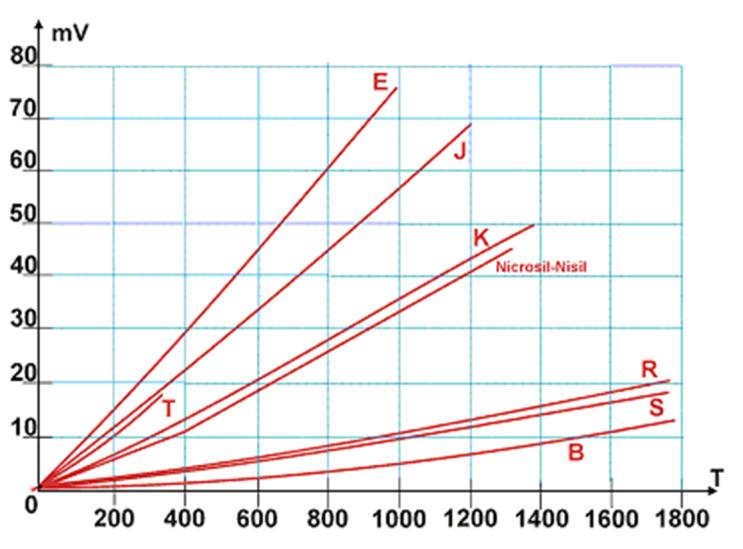
\includegraphics[scale=0.6]{figuras/fig-thermocouple-output.jpg}
		\caption{Thermocouple characteristic voltage output \cite{termo-curves}}
		\label{fig:thermocoupleVoltage}
	\end{figure}
		
	Thermocouple actually have two junctions, a hot junction (the one that is submitted to heat transfers) and a cold junction (also called reference junction). What the thermocouple really measures is the difference between the temperature of this two junctions, this means that in a hypothetical situation which the hot junction is submmited to a 100$^{\circ}$C and the cold junction is submitted to a environmental temperature of 25$^{\circ}$C, after thermal equilibrium is reached the thermocouple voltage will be proportional to a temperature of 75$^{\circ}$C. Hence the thermocouple will only produce a "real" output voltage when the cold junction is submitted to a 0$^{\circ}$C (in some calibrations procedures the cold junction is actually submitted to 0$^{\circ}$C) \cite{kinzie1973thermocouple}.
		
	\begin{figure}[htbp]
		\centering
			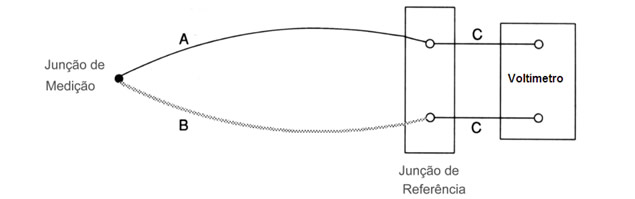
\includegraphics[scale=0.75]{figuras/fig-thermocouple-measurement.jpg}
		\caption{Thermocouple Measurement \cite{termo-med}}
		\label{fig:thermocoupleMeasurement}
	\end{figure}
		
	There is a big variety of thermocouples available, table \ref{table:thermocouple} shows the most common thermocouples and there temperature range.

	\begin{table}[h!]
		\centering
		\caption{Thermocouples and their operation ranges}
		\label{table:thermocouple}
		\begin{tabular}{|c|c|}
			\hline
			\textit{\textbf{Thermocouple Type}} & \textit{\textbf{Range of Operation ($^{\circ}$C)}} \\ \hline
			J & 0 a 750 \\ \hline
			K & -200 a 1250 \\ \hline
			E & -200 a 900 \\ \hline
			T & -250 a 350 \\ \hline
		\end{tabular}
	\end{table}
